
%il reste à faire une partie sur les applications affines







\subsubsection{Changement d'orientation de caméra :}
On étudie ici un cas particulier d'homographie $h$   que l'on peut interpréter comme un changement d'angle de caméra.\\
\begin{figure}[h!]
\centering
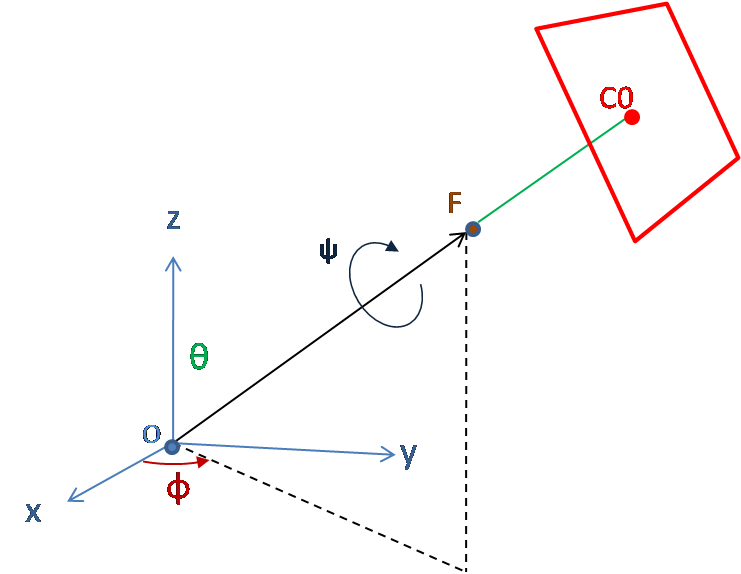
\includegraphics[width=10cm]{shema_decomp.png}
\caption{Illustration d'un changement d'angle de caméra $(X_v =0)$}
\end{figure}

\paragraph{Approche géométrique :}
\subparagraph{Cas général :}
On se place dans l'espace $\mathbb{R}^{3}$,on le munit d'une base orthonormale directe $(x_{0},y_{0},z_{0})$,\\ l'image de départ sera située dans le plan $P_{1}= \mathbb{R}^{2}\times \{0\}$.\\
On doit maintenant positionner notre caméra par rapport à l'image de départ.
\begin{itemize}
\item On note $F$ la position de l'objectif de la caméra, et $w$ le vecteur directeur unitaire de l'axe optique de la caméra. L'axe optique de la caméra est donc la droite passant par $F$ et dirigée par $w$.
\item On note $\delta$ la distance entre l'objectif et l'écran.
\item L'écran $P_{2}$ est alors le plan affine passant par $F+\delta w$ et perpendiculaire à l'axe optique de la caméra.
\begin{equation*}
P_{2}=\{Y\in \mathbb{R}^{3}|(Y-F-\delta w)\cdot w=0\}=\{Y\in \mathbb{R}^{3}|(Y-F)\cdot w=\delta\}
\end{equation*}
\end{itemize}

On définit l'application $H$ qui à un point $X\in P_{1}$ lui associe sa projection homographique sur $P_{2}$. C'est-à-dire que le point $H(X)$ est le point d'intersection entre la droite $D_{X}$ (passant par $X$ et $F$) et le plan $P_{2}$.\\
Cette application n'est pas définie sur $P_{1}$ tout entier, comme $D_{X}=\{X+t(F-X)|t\in\mathbb{R}\}~~~$, si $H(X)$ existe alors 
\begin{equation*}
\exists t_{X}~~~~H(X)=X+t_{X}(F-X)
\end{equation*}
Comme $H(X)\in P_{2}$ alors
\begin{equation*}
(H(X)-F)\cdot w =\delta
\end{equation*}
Et donc 
\begin{equation*}
t_{X}=1+\frac{\delta}{w\cdot(F-X)}
\end{equation*}
Finalement on en déduit que l'application $H$ est définie sur $P_{1}'=P_{1}\backslash \{Y\in P_{1}|w\cdot(F-Y)=0\}$ et 
\begin{equation*}
H(X)=Z+\delta w+\delta \frac{(F-X)-(F-X)\cdot w~ w}{w\cdot (F-X)}
\end{equation*}

\subparagraph{Introduction du point visé :}
On se place dans le cas où le vecteur $w$ n'appartient pas à $P_{1}$ dans se cas on peut définir $X_{v}$ le point de $P_{1}$ visé par la caméra, c'est-à-dire le point d'intersection entre l' axe optique et le plan $P_{1}$.On obtient alors 
\begin{equation*}
X_{v}=F-\delta'w~~~~~~\delta'=\small{\left|\frac{F \cdot z_{0}}{w\cdot z_{0}} \right|}
\end{equation*}
On peut alors en déduire que l'application $H$ est définie sur\\ $P_{1}'=P_{1}\backslash \{Y\in P_{1}|\delta'+w\cdot(X_{v}-Y)=0\}$ et 
\begin{equation*}
H(X)=X_{v}+(\delta+\delta')w+\delta_{2}\frac{(X_{v}-X)-(X_{v}-X)\cdot w~ w}{\delta'+w\cdot (X_{v}-X)}
\end{equation*}



\subparagraph{Formulation analytique :}

L'application $H$ est une application de $P_{1}'$ dans $P_{2}$. Pour construire une expression analytique du changement d'angle de caméra on peut munir le plan $P_{1}$ de la base $(x_{0},y_{0})$, de même le plan affine $P_{2}$ peut être munit d'un repère orthonormé $(C,u,v)$ tel la famille $(u,v,w)$ soit un base orthonormale directe de $\mathbb{R}^{3}$, et que le point $C$ soit un point quelconque de l'écran qui servira d'origine.\\
On peut repérer le point $C$ par rapport au centre de l'écran $C_{0}$ c'est-à-dire la projection orthogonale de l'objectif sur l'écran $C_{0}=Z+\delta w$ et $C=C_{0}+c_{u}u+c_{v}v$.\\
On peut alors définir les applications $i$ et $k$
\begin{itemize}
\item $i:\mathbb{R}^{2}\rightarrow P_{1}$~~~~$i((x,y))=x~x_{0}+y~y_{0}$
\item $k:P_{2}\rightarrow \mathbb{R}^{2}$~~~~$k(X)= ((X-C)\cdot u~,~(X-C)\cdot v)=((X-F)\cdot u-c_{u}~,~ (X-F)\cdot v-c_{v})$
\end{itemize}
On pose alors 
\begin{equation*}
h=k\circ H \circ i
\end{equation*}
h est une application définie sur $\mathbb{R}^{2}$ privé d'une droite. On obtient dans le cas général
\begin{equation*}
\forall X\in \mathbb{R}^{2} ~~~~~h(X)=\left(\frac{\delta (F-i(X))\cdot u}{w \cdot (F-i(X))}-c_{u}~,~\frac{\delta (F-i(X))\cdot v}{w \cdot (F-i(X))} -c_{v} \right) 
\end{equation*} 
Dans le cas où le point visé existe
\begin{equation*}
\forall X\in \mathbb{R}^{2} ~~~~~h(X)=\left(\frac{\delta (X_{v}-i(X))\cdot u}{w \cdot (X_{v}-i(X))+\delta'}-c_{u}~,~\frac{\delta (X_{v}-i(X))\cdot v}{w \cdot (X_{v}-i(X))+\delta'} -c_{v} \right) 
\end{equation*}



\paragraph{Décomposition de l'homographie h dans le cas où le point visé existe :}
%tu identifie une rotation et son angle, c'est etrange
Le vecteur $w$, on peut le positionner par rapport au repère $(x_{0},y_{0},z_{0}) $ en introduisant deux angles, $\phi$ et $\theta$
\begin{itemize}
\item la première rotation d'angle $\phi$ se fait autour de l'axe $z_{0}$ on lui associe la base $(x_{1},y_{1},z_{1})$ où $z_{0}=z_{1}$.
\item la seconde rotation d'angle $\theta$ se fait autour de l'axe $y_{1}$ on lui associe la base $(x_{2},y_{2},z_{2})$ où $z_{2}=w$ et $y_{1}=y_{2}$.
\end{itemize}
\begin{figure}[h!]
\centering
\subfigure[rotation $\phi$]{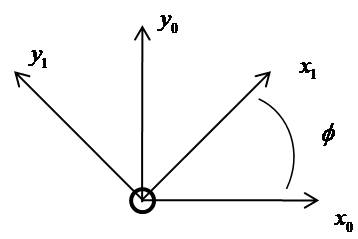
\includegraphics[width=5cm]{graphe1.jpg}}
\subfigure[rotation $\theta$]{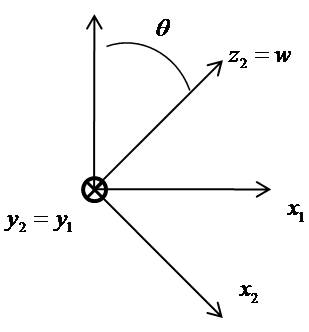
\includegraphics[width=5cm]{graphe2.jpg}}

\end{figure}
Pour positionner la caméra on doit définir sa rotation propre autour de son axe optique pour cela on définit l'angle $\psi$.\\
\begin{figure}[h!]
\centering
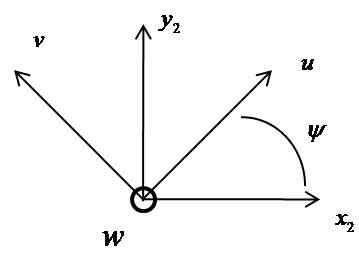
\includegraphics[width=5cm]{graphe3.jpg}
\caption{rotation propre}
\end{figure}
On obtient alors 
\begin{equation*}
u=\cos(\psi)x_{2}+\sin(\psi)y_{2}~~~~~~~~~~v=-\sin(\psi)x_{2}+\cos(\psi)y_{2}
\end{equation*}
Si on pose $R_{s}$ la rotation d'angle $s$ et $\tau_{y}$ la translation de vecteur $-y$ on obtient alors 
\begin{equation*}
(\tau_{c}^{-1} \circ h)(X) = R_{\psi}\left(\frac{\delta (X_{v}-i(X))\cdot x_{2} }{w \cdot (X_{v}-i(X))+\delta'}~,~\frac{\delta (X_{v}-i(X))\cdot y_{2}}{w \cdot (X_{v}-i(X))+\delta'}  \right) 
\end{equation*}
On assimile $X_{v}$ et $i^{-1}(X_{v})$ on obtient 
\begin{equation*}
(R_{\psi}^{-1} \circ \tau_{c}^{-1}  \circ h)(X)=\left(\frac{-i(\tau_{x_{v}} (X))\cdot x_{2} }{-w \cdot i(\tau_{x_{v}} (X))+\delta'}~,~\frac{-i(\tau_{x_{v}} (X))\cdot y_{2}}{-w \cdot i(\tau_{x_{v}} (X))+\delta'}  \right) 
\end{equation*}

Comme $z_{2}=cos(\theta)z_{1}+sin(\theta)x_{1}~~x_{2}=cos(\theta)x_{1}-sin(\theta)z_{1}~$ et $z_{1}\perp P_{1}$ alors

\begin{equation*}
(R_{\psi}^{-1} \circ \tau_{c}^{-1}  \circ h)(X)=\left(\frac{-\cos(\theta)i(\tau_{x_{v}} (X))\cdot x_{1} }{\delta'-\frac{sin(\theta}{\delta'}x_{1}\cdot i(\tau_{x_{v}}(X))}~,~\frac{-i(\tau_{x_{v}} (X))\cdot y_{1}}{\delta'-\frac{sin(\theta}{\delta'}x_{1}\cdot i(\tau_{x_{v}}(X))}  \right) 
\end{equation*}

Si on note $h_{\theta,\delta'}$ 

\begin{equation*}
h_{\theta,\delta'}(x',y')=\left(\frac{-cos(\theta)x'}{1-\frac{sin(\theta)}{\delta'}x'} ~,~\frac{-y'}{1-\frac{sin(\theta)}{\delta'}x'}\right)
\end{equation*}

Alors 

\begin{equation*}
(R_{\psi}^{-1} \circ \tau_{c}^{-1} h)(X)= \frac{\delta}{\delta'}h_{\theta,\delta'}\left ( i(\tau_{x_{v}}(X)) \cdot x_{1}~,~ i(\tau_{x_{v}}(X)) \cdot y_{1}\right)
\end{equation*}

Comme $x_{1}=\cos(\phi)x_{0}+\sin(\phi)y_{0}~~~y_{1}=-\sin(\phi)x_{0}+\cos(\phi)y_{0}$ alors

\begin{eqnarray*}
(R_{\psi}^{-1} \circ \tau_{c}^{-1} \circ h)(X) &=& \frac{\delta}{\delta'}h_{\theta,\delta'}\left ( R_{\phi}(i(\tau_{x_{v}}(X)) \cdot x_{0}~,~ i(\tau_{x_{v}}(X)) \cdot y_{0})\right)\\
                                               &=&\frac{\delta}{\delta'} (h_{\theta,\delta'}\circ R_{\phi} \circ \tau_{x_{v}})(X)
\end{eqnarray*}

Si

\begin{equation*}
z_{\lambda}:X\rightarrow \lambda X
\end{equation*}

On obtient la formule générale pour les changements d'angle de caméra
\begin{prop}  $h$ est un changement d'angle de caméra si et seulement si existe des paramètres $(\delta,\delta',\theta,\phi,\psi,C,X_v)$ tels que :
\begin{equation}
h= \tau_{c} \circ z_{\frac{\delta}{\delta'}}  \circ R_{\psi} \circ h_{\theta,\delta'} \circ R_{\phi} \circ \tau_{x_{v}}
\label{formul_decomp}
\end{equation}
\end{prop



\subsubsection{Application à la décomposition des homographies :}
\paragraph{Résultats généraux sur les homographies :}
 On rappelle ici les notions sur les homographies qui nous seront utiles dans la suite. Le lien entre les homographies et les espaces projectifs ne sera pas étudié. Dans toute la suite du document, une homographie $h$ est une application injective de la forme :
	\[h:(x,y)\mapsto \left(\frac{ax+by+p}{rx+sy+t},\frac{cx+dy+q}{rx+sy+t}\right)\]
Les applications affines sont un cas particulier d'homographie, si une homographie n'est pas une application affine alors elle est définie sur le plan privé d'une droite appelée horizon.\\	
  L'ensemble des homographies a une structure de groupe pour la loi de composition .\\
  On peut  associer à l'homographie $h$ la matrice $H$ définies par
  
	\begin{equation*}
	H=\begin{pmatrix}
	a&b&p\\c&d&q\\r&s&t
	\end{pmatrix}
	\end{equation*}
	Cette matrice est inversible car $h$ est inversible, elle n'est pas unique car la matrice $\lambda H$ définit la même homographie $\forall \lambda \in \mathbb{R}_+$.\\
Cette notation rend compatible le produit matriciel et la composition des homographies. On obtient un morphisme de groupe de $GL_{3}(\mathbb{R})$ dans le groupe des homographies du plan. Ce morphisme n'est pas injectif, la matrice d'une homographie est définie à proportionnalité près mais il se quotiente à travers $SL_{3}(\mathbb{R})$ en un isomorphisme.\\
Dans la suite on notera $\sim$ la relation d'équivalence  sur $GL_{3}(\mathbb{R})$ définie par $A\sim B \iff \exists \lambda\in \mathbb{R}^{*} , A=\lambda B$, c'est-à-dire si $A$ et $B$ définissent la même homographie.\\
\underline{Remarque :} Dans certains cas une homographie peut être définie par ses valeurs prises en quatre points du plan.\\



\paragraph{Décomposition matricielle :}
\begin{prop}
Toute homographie est un mouvement de caméra où une application affine. Dans le premier cas la décomposition \ref{formul_decomp} n'est pas unique possède un degrés de liberté.
\end{prop}
%la ref n'apparait pas bien
On fixe $h$ une homographie et $H$ une matrice qui lui est associée. On conserve ici les notations de la partie précédente, on suppose sans perte de généralité que $\det (H)=1$. On suppose de plus que $h$ peut s'écrire sous la forme $\ref{formul_decomp}$, on cherche à montrer que cette hypothèse n'impose aucune condition supplémentaire sur la matrice $H$, en déterminant les paramètres intervenants dans la décomposition en fonction des coefficients de $H$ .\\
On a la formule de décomposition :

\begin{equation*}
h=z_{\frac{\delta}{\delta'}} \circ \tau_{c}\circ R_{\psi} \circ h_{\theta,\delta'} \circ R_{\phi} \circ \tau_{x_{v}}
\end{equation*}
Chacune de ces transformations est une homographie, on peut donc réécrire cette relation en utilisant des matrices. On obtient 
 \begin{equation*}
H\sim T_{c} Z_{\frac{\delta}{\delta'}}  R_{\psi}  H_{\theta,\delta'} R_{\phi}  T_{x_{v}}
\end{equation*}
\begin{equation*}
R_{\alpha}=\begin{pmatrix}
\cos(\alpha)&\sin(\alpha)&0\\-\sin(\alpha)&cos(\alpha)&0\\0&0&1
\end{pmatrix}
~~~~H_{\theta,\delta'}=\begin{pmatrix}
-\cos(\theta)&0&0\\0&-1&0\\-\frac{\sin(\theta)}{\delta'}&0&1
\end{pmatrix}
\end{equation*}
\begin{equation*}
~~~~Z_{\lambda}=\begin{pmatrix}
\lambda&0&0\\0&\lambda&0\\0&0&1
\end{pmatrix}
~~~~T_{X_{v}}=\begin{pmatrix}
1&0&-x_{v}\\0&1&-y_{v}\\0&0&1
\end{pmatrix}
\end{equation*}
 On cherche dans un premier temps à déterminer les translations. Soient $X_1 = (x_1 , y_1 )$ et $X_2 = (x_2 , y_2 )$ deux vecteurs que l'on suppose tel que la matrice $H_t$ définie par $H_t = T_{-X_2}  \cdot H \cdot T_{X_1}$ admette une décomposition de la forme  $H_t=R_{\psi} \cdot H_{\theta,\delta} \cdot R_{\phi}$ .\\
 On pose 
 \begin{equation*}
 H^{-1}=\begin{pmatrix} A&B&P\\C&D&Q\\R&S&T \end{pmatrix}
 \end{equation*}
 Par un calcul on obtient que la matrice $R_{\psi} \cdot H_{\theta,\delta} \cdot R_{\phi}$ est égale à : 
  \begin{equation*}
\begin{pmatrix}
 -\frac{\delta}{\delta'}\cos(\psi)\cos(\theta)\cos(\phi)+\frac{\delta}{\delta'}\sin(psi)\sin(\phi)& -\frac{\delta}{\delta'}\cos(\psi)\cos(\theta)\sin(\phi)-\frac{\delta}{\delta'}\sin(\psi)\cos(\phi)&0\\
  \frac{\delta}{\delta'}\sin(\psi)\cos(\theta)\cos(\phi)+\frac{\delta}{\delta'}\cos(\psi)\sin(\phi)& \frac{\delta}{\delta'}\sin(\psi)\cos(\theta)\sin(\phi)-\frac{\delta}{\delta'}\cos(\psi)\cos(\phi)&0\\ -\frac{\sin(\theta)}{\delta'}\cos(\phi)&-\frac{\sin(\theta)}{\delta'}\sin(\phi)& 1
 \end{pmatrix}
 \end{equation*}
 On a de plus 
 \begin{equation*}
 H_t=\begin{pmatrix}
 a-x_2 r&b-x_2 s& a x_1 + b y_1 + p -x_2 (r x_1 +s y_1 +t)\\
  c-y_2 r&d-y_2 s& c x_1 + d y_1 + q -y_2 (r x_1 +s y_1 +t)\\
  r & s & r x_1 + s y_1 +t
 \end{pmatrix}
 \end{equation*}
 On a donc l'équivalence 
 \begin{equation*}
 (H_t)_{1,3}=(H_t)_{2,3}=0 \iff (x_2,y_2)=h(x_1,y_1) \iff (x_1,y_1)=h^{-1}(x_2,y_2)
 \end{equation*}
 On pose $(x_1,y_1)=h^{-1}(x_2,y_2)$ car les calculs intermédiaires sont moins fastidieux, on suppose $(x_2,y_2)$ tels que $R x_2 +S y_2 + T \ne 0$.\\
On obtient alors
\begin{equation*}
H_t
  \sim 
  \begin{pmatrix}
 (a-x_2 r)(R x_2 + S y_2 +T)&(b-x_2 s)(R x_2 + S y_2 +T)& 0\\
  (c-y_2 r)(R x_2 + S y_2 +T)&(d-y_2 s)(R x_2 + S y_2 +T)& 0\\
  r(R x_2 + S y_2 +T) & s(R x_2 + S y_2 +T) &1
  \end{pmatrix} 
\end{equation*}
On obtient alors 
 \begin{equation*}
 -\frac{\sin(\theta)}{\delta'}\cos(\phi)=r(R x_2 + S y_2 +T)~~~~~~ -\frac{\sin(\theta)}{\delta'}\sin(\phi)=s(R x_2 + S y_2 +T)
 \end{equation*}
 On sait que $r^{2}+s^{2}=0$ si et seulement si l'homographie associée à H est une affinité. Ce cas ci sera traité de façon indépendante, on suppose ici que l'homographie $h$ n'est pas une affinité. On peut donc écrire :
 \begin{eqnarray*}
 \cos(\psi) &=& \sgn\left(-\frac{\sin(\theta)}{ \delta'}\right)\sgn(R x_2 + S y_2 +T)\frac{r}{\sqrt{r^{2}+s^{2}}}\\
 \sin(\psi) &=& \sgn\left(-\frac{\sin(\theta)}{ \delta'}\right)\sgn(R x_2 + S y_2 +T)\frac{s}{\sqrt{r^{2}+s^{2}}}
 \end{eqnarray*}
 On peut se restreindre au cas $\frac{\sin(\theta)}{\delta'}>0$ :\\
 \begin{itemize}
 \item En effet si $\frac{\sin(\theta)}{\delta'}<0$ on obtient alors
 \begin{equation*}
 R_{\psi} \cdot H_{\theta,\delta'} \cdot R_{\phi}=R_{\psi} \cdot Z_{-1}\cdot H_{\theta,-\delta'}\cdot Z_{-1} \cdot R_{\phi}= R_{\psi+\pi} \cdot H_{\theta,-\delta'}\cdot R_{\phi+\pi}
 \end{equation*}
 et on a $-\frac{\sin(\theta)}{\delta'}>0$.\\
 \end{itemize}


 On obtient alors 
 \begin{equation*}
 \cos( \phi )= -\sgn(R x_2 +S y_2 +T) \frac{r}{\sqrt{r^2 + s^2}}~~~~~~ \sin( \phi )= -\sgn(R x_2 +S y_2 +T) \frac{s}{\sqrt{r^2 + s^2}}
 \end{equation*}
 Comme 
 \begin{equation*}
H_t \cdot R_{\phi}^{-1} \sim
 \begin{pmatrix}
 -|R x_2 +S y_2 +T|\frac{(ar+sb)-(r^2 + s^2)x_2}{\sqrt{r^2 + s^2}}&-|R x_2 +S y_2 +T|\frac{S}{\sqrt{r^2 + s^2}}&0\\
 -|R x_2 +S y_2 +T|\frac{(cr+sd)-(r^2 + s^2)y_2}{\sqrt{r^2 + s^2}}&|R x_2 +S y_2 +T|\frac{r}{\sqrt{r^2 + s^2}}&0\\
 -|R x_2 +S y_2 +T|\sqrt{r^2 + s^2}&0&1
 \end{pmatrix}
 \end{equation*}
 Et d'un autre côté 
 \begin{equation*}
R_{\psi} \cdot H_{\theta,\delta}  \sim 
 \begin{pmatrix}
 -\frac{\delta}{\delta'}\cos(\psi)\cos(\theta)&
-\frac{\delta}{\delta'}\sin(\psi)&
0\\
\frac{\delta}{\delta'}\sin(\psi)\cos(\theta)&
-\frac{\delta}{\delta'}\cos(\psi)&
0\\
-\frac{\sin(\theta)}{\delta'}&
0&
1
 \end{pmatrix}
 \end{equation*}
Comme $h$ n'est pas une affinité on a $R^2 + S^2 \ne 0$ 
 \begin{equation*}
  \cos( \psi ) =- \sgn(\frac{\delta}{\delta'})\frac{R}{\sqrt{R^2 + S^2}}~~~~~~ \sin( \psi ) = \sgn(\frac{\delta}{\delta'})\frac{S}{\sqrt{R^2 + S^2}}
 \end{equation*}
On peut se restreindre au cas $\frac{\delta}{\delta'}>0$ :\\
\begin{itemize}
\item En effet si $\frac{\delta}{\delta'}<0$ on obtient alors $Z_{\frac{\delta}{\delta'}} \cdot R_{\psi}=Z_{\left|\frac{\delta}{\delta'}\right|}\cdot Z_{-1} \cdot R_{\psi}=Z_{\left|\frac{\delta}{\delta'}\right|}\cdot R_{\pi} \cdot R_{\psi}=Z_{\left|\frac{\delta}{\delta'}\right|}\cdot R_{\psi+\pi}$.
\end{itemize}
Et donc 
 \begin{equation*}
  \cos( \psi ) =- \frac{R}{\sqrt{R^2 + S^2}}~~~~~~ \sin( \psi ) = \frac{S}{\sqrt{R^2 + S^2}}
 \end{equation*}



 On obtient alors 
\begin{equation*}
R_{\psi}^{-1} \cdot H_t \cdot R_{\phi}^{-1} \sim 
 \begin{pmatrix}
 -|R x_2 +S y_2 +T|(R x_2 +S y_2 +T)\sqrt{\frac{r^2 + s^2}{R^2 + S^2}}&0&0\\
 |R x_2 +S y_2 +T|\frac{\Delta(x_2 , y_2)}{\sqrt{r^2 + s^2}\sqrt{R^2 + S^2}}&-|R x_2 +S y_2 +T|\sqrt{\frac{R^2 + S^2}{r^2 + s^2}}&0\\
 -|R x_2 +S y_2 +T|\sqrt{r^2 + s^2}&0&1
 \end{pmatrix}
\end{equation*}
Où l'on a posé 
\begin{equation*}
\Delta(x_2 , y_2 ) =R ((rc+sd)-(r^2 + s^2)y_2) - S ((ar+sb)-(r^2 + s^2 )x_2)
\end{equation*}
On obtient alors $\Delta(x_2 , y_2 )=0$ si et le seulement il existe $\lambda$ tel que  %j'aime pas le il existe comme ça...
\begin{equation*}
x_2=\frac{ar+sb+R \lambda}{r^2 +s^2}~~~~y_2=\frac{cr+sd+S \lambda}{r^2 +s^2}
\end{equation*}
On a de plus 
\begin{equation*}
R x_2 +S y_2 +T = \frac{R^2 +S^2}{r^2 + s^2} \lambda
\end{equation*}
Le paramètre $\lambda$ doit donc être pris différent de zéros 
\begin{equation*}
R_{\phi}^{-1} \cdot H_t \cdot R_{\psi}^{-1} \sim 
 \begin{pmatrix}
 -| \lambda | \lambda \sqrt{\frac{R^2 + S^2}{s^2 + r^2}}^{3}&0&0\\
0&-| \lambda | \sqrt{\frac{R^2 + S^2}{r^2 + s^2}}^{3}&0\\
 -|\lambda|\frac{R^2 + S^2}{\sqrt{r^2 + s^2}}&0&1
 \end{pmatrix}
\end{equation*}
 
 
 On peut poser 
 \begin{equation*}
 \frac{\delta}{\delta'}=|\lambda|\sqrt{\frac{R^2 + S^2}{r^2 + s^2}}^{3}
 \end{equation*}
On obtient finalement
\begin{equation*}
Z_{\frac{\delta}{\delta'}}^{-1} \cdot R_{\phi}^{-1} \cdot H_t \cdot R_{\psi}^{-1} \sim 
 \begin{pmatrix}
 -\lambda&0&0\\
0&-1&0\\
 -|\lambda|\frac{R^2 + S^2}{\sqrt{r^2 + s^2}}&0&1
 \end{pmatrix}
 \end{equation*}
 Cette matrice doit être de la forme $H_{\theta,\delta'}$ on doit avoir 
 \begin{equation*}
 \lambda^2 + \lambda^2 \delta'^2 \frac{(R^2 + S^2)^2}{r^2 + s^2}=1 ~~~~\iff \delta'^2 = (r^2 + s^2) \frac{1-\lambda^2}{\lambda^2 (R^2+S^2)^2}
 \end{equation*}
 
 \paragraph{Synthèse et optimisation :}
 On a montré dans la section précédente que toute homographie qui n'est pas une application affine est un changement d'angle de caméra. On a de plus que pour tout $\lambda \in ]0,1[$ %pas certain que c'est ce que tu veux dire
 \begin{equation*}
x_2=\frac{ar+sb+R \lambda}{r^2 +s^2}~~~~y_2=\frac{cr+sd+S \lambda}{r^2 +s^2}~~~~(x_1 , y_1) = h^{-1}(x_{2},y_{2})
\end{equation*}
 \begin{equation*}
 \cos( \phi )= - \frac{r}{\sqrt{r^2 + s^2}}~~~~ \sin( \phi )= - \frac{s}{\sqrt{r^2 + s^2}}~~~~\cos( \psi ) =- \frac{R}{\sqrt{R^2 + S^2}}~~~~ \sin( \psi ) = \frac{S}{\sqrt{R^2 + S^2}}
 \end{equation*}
 \begin{equation*}
 \frac{\delta}{\delta'}=|\lambda|\sqrt{\frac{R^2 + S^2}{r^2 + s^2}}^{3}~~~~\cos(\theta)=\lambda~~~~\sin(\theta)=\sqrt{1-\lambda^2}~~~~\delta'=  \frac{\sqrt{(r^2 + s^2)(1-\lambda^2)}}{|\lambda| (R^2+S^2)}
 \end{equation*}
 Le degré de liberté correspond à une translation en sortie dans une direction perpendiculaire à l'horizon de $H^{-1}$.\\
 Une décomposition plus générale autorise $\lambda \in \mathbb{R}^{*}$.
